\section{Demonstration}
In this section, we detail the proposed demonstration.
The objective of this demonstration is to illustrate 
how \sys can improve iterative process of data analysis.
Data scientists often have to work with multiple but related dirty datasets.
If a data scientist optimizes a data cleaning pipeline on one dataset, with \sys 
she quickly transfer those insights to develop a pipeline on the other.

\subsection{Datasets}
In our demo, we will consider entity resolution tasks in two different restaurant datasets.
In first dataset contains 858 Zagat reviews \footnote{\scriptsize{ \url{http://www.cs.utexas.edu/users/ml/riddle/data/restaurant.tar.gz}}},
and tags each restaurant with a category such as ``Chinese" or ``American".
These categories are inconsistent across records e.g, ``Chinese" and ``Chinese Cuisine".
The second dataset is from Yelp and contains 58,127 restaurant records that are also tagged with a category.
The category attribute is inconsistent in similar ways to the Zagat reviews.
We will use \sys to merge similar categories together and find the top 10 most popular categories in the dataset.

\begin{figure}[t]
\centering
 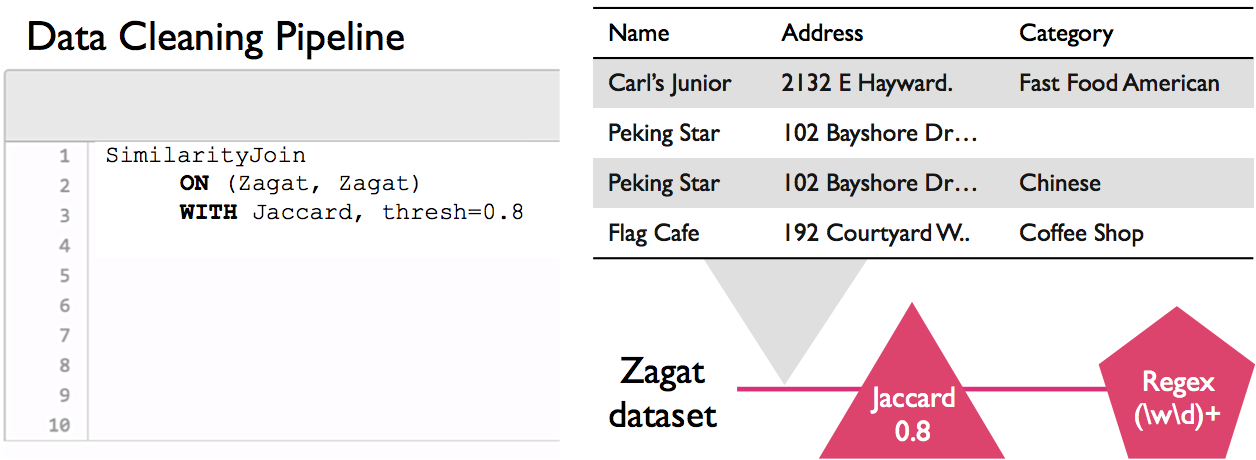
\includegraphics[width=0.75\columnwidth]{figs/dashboard_screenshot.png}
 \caption{The dashboard contains both a visual interface and a text box to specify the data cleaning operation. When the user is satisfied, she can run the plan and see the results on the right. \label{screenshot}}
\end{figure}


\begin{figure}[t]
\centering
 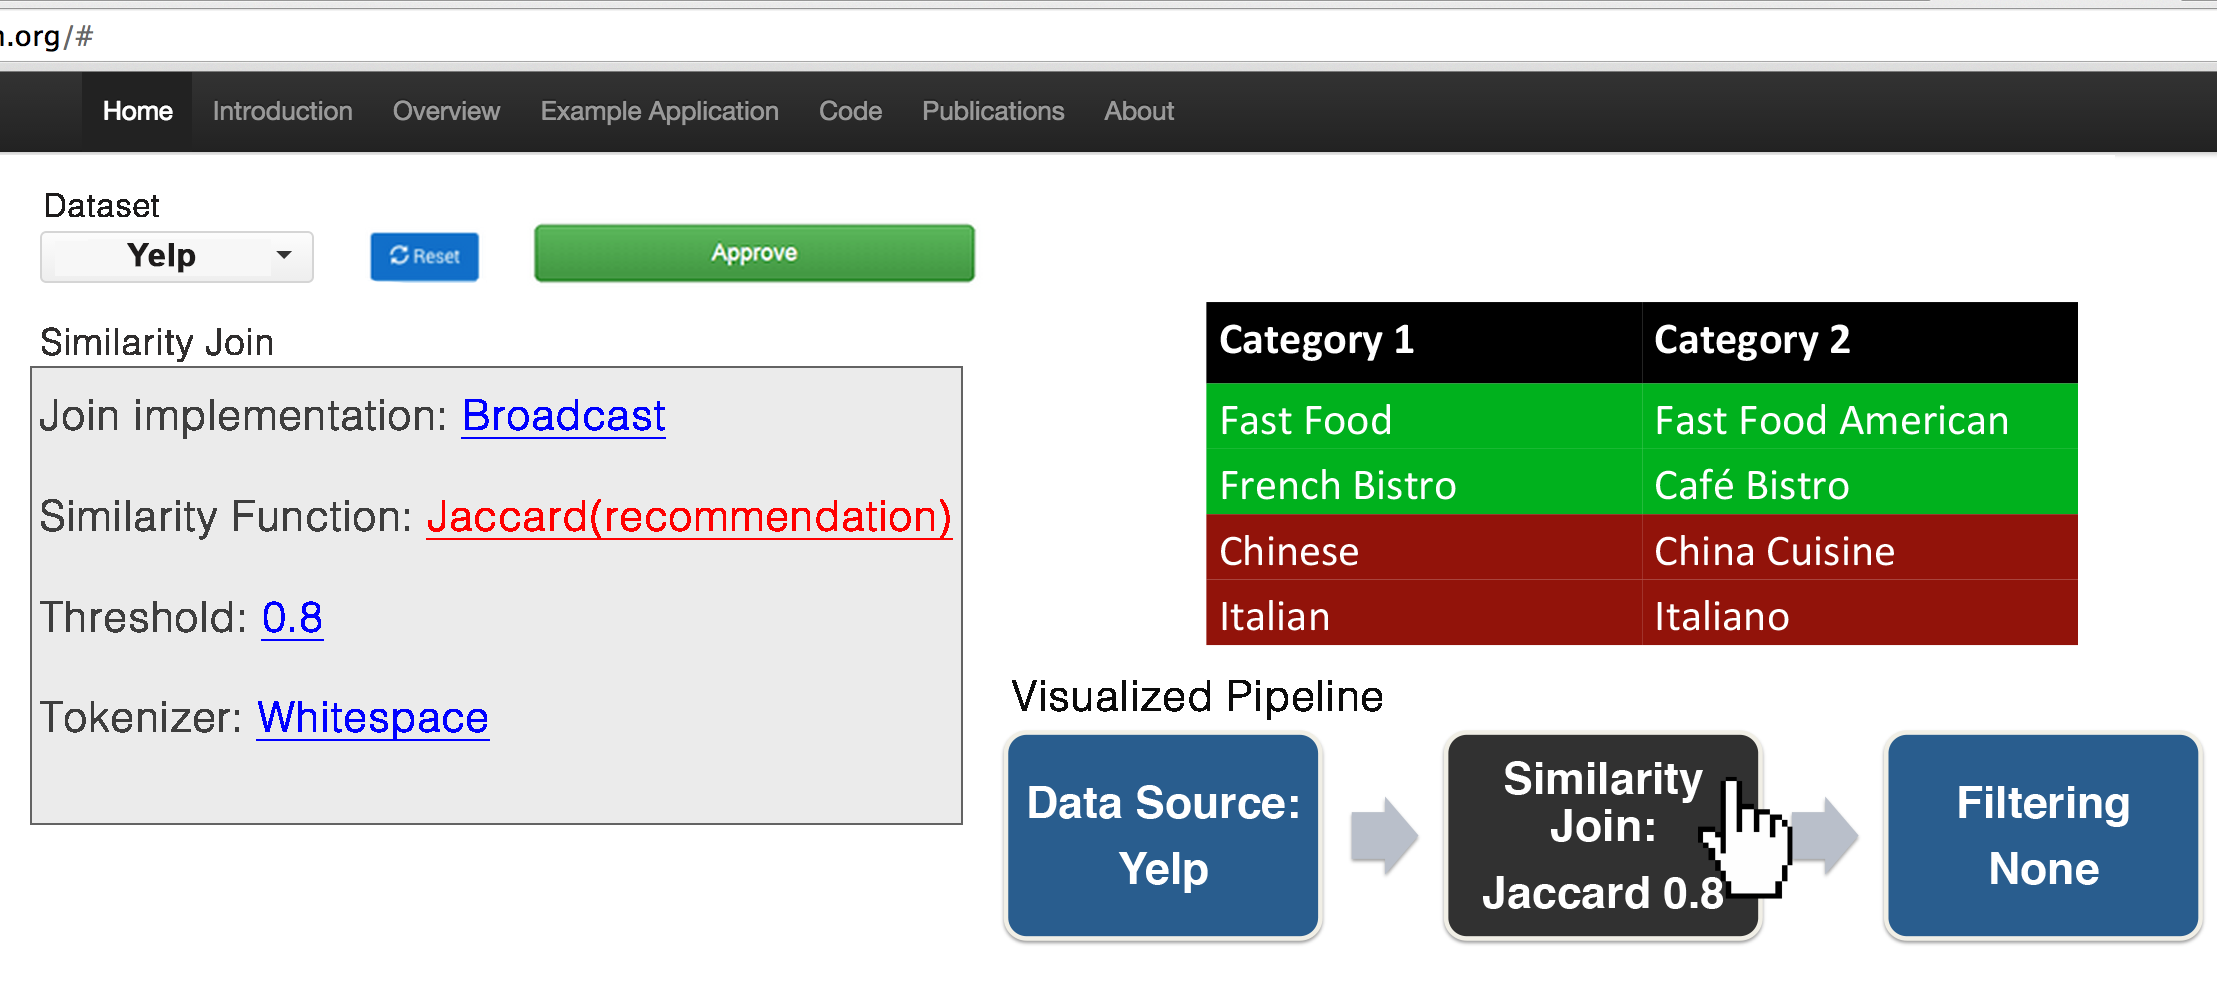
\includegraphics[width=0.65\columnwidth]{figs/dashboard_recsys.png}
 \caption{The operator view lists the parameters of the operator. Users can change parameters on the fly and can also see recommended changes. \label{screenshot-rec}}\vspace{-1.75em}
\end{figure}

\subsection{Demo Walkthrough}
Now, we will detail the steps of the proposed demonstration.
A screenshot of our dashboard interface is illustrated in Figure \ref{screenshot}.

\vspace{0.5em}

\noindent\textbf{Step 1: } We will explain the components of our dashboard interface to the
demo participants. We will explain how to design data cleaning plans with the visual 
drop down menus, how to compile those plans to our DSL, and how to evaluate the results.

\vspace{0.5em}

\noindent\textbf{Step 2: } Our dashboard will be pre-populated with a data cleaning specification from Section~\ref{s:apps}, and will
start off with the Zagat restaurant dataset. With the visual interface participants will have the option of choosing one of two Similarity Join implementations, Edit Distance and Jaccard Similarity, and they can tune the threshold.
Participants can also add a crowdsourced filtering step in addition to the similarity thresholding. 

\vspace{0.5em}

\noindent\textbf{Step 3: } When a participant is satisified with a plan, they can hit ``Approve" and it will execute the data cleaning. If they chose to use crowdsourcing, then they can complete crowd tasks. The results of the plan are visualized in the upper right of our interface.
We show a representative sample of changed records allowing the partipcant to understand how the cleaning affects the data. 
Participants can further analyze their plan by clicking on an operator (Figure \ref{screenshot-rec}).
In addition to the parameters, this shows the recommended changes to the operator.
For example, in Figure \ref{screenshot-rec}, we show a recommendation to change the similarity metric from Jaccard to Edit Distance since the attribute in question does not have many tokens.

\vspace{0.5em}

\noindent\textbf{Step 4: } Participants can then change datasets and observe how the same pipeline would work on another dataset.
They can modify the plan using the visual interface until the results are satisfactory.

\if{0}
\subsection{1. Cleaning}
VLDB attendees will specify the data cleaning operations with an interactive browser based
interface. 

\subsection{2. Code}
VLDB attendees can see the generated code from the browser interface.

\subsection{3. Crowd Tasks}
VLDB attendees perform any generated crowd tasks from the code.  

\subsection{3. Progressive Result Visualization}
VLDB attendees can see the results change in real time.  
\fi
